\documentclass[a4paper]{report}
\usepackage[14pt]{extsizes} % для 14 размера шрифта

\usepackage{setspace}
\usepackage[left=20mm, top=15mm, right=15mm, bottom=15mm, nohead, footskip=10mm]{geometry} % настройки полей документа

\usepackage[utf8]{inputenc}
\usepackage[english, russian]{babel}
\usepackage{indentfirst}
\usepackage[hidelinks]{hyperref}
\hypersetup{
    allcolors=black
}

\usepackage{amsmath} % для математических формул и для автоматического добавления скобок при цитировании
\usepackage{physics} % Для дифференцирования
\usepackage{IEEEtrantools} % для создания многострочных математических формул
\usepackage{mathtools} % для знака модулю для дроби

\usepackage[justification=centering]{caption} % подписи таблиц посередине

\newcommand{\No}{\textnumero} % для значка №
% для подписи под пределом
\newcommand{\Lim}[1]{\raisebox{0.5ex}{\scalebox{0.8}{$\displaystyle \lim_{#1}\;$}}}
\DeclarePairedDelimiter\Abs{\lvert}{\rvert} % для знака модуля для дроби

% \graphicspath{{./figs/}}

\begin{document}

\begin{titlepage}

\begin{center}
    Министерство образования и науки Российской Федерации\\
    Федеральное государственное автономное образовательное учреждение\\
    высшего образования\\
    <<Санкт-Петербургский политехнический университет Петра Великого>>
\end{center}

\vfill

\begin{center}
    КУРСОВАЯ РАБОТА\\
    по теме:\\
    <<Теория возмущений. Метод асимптотических возмущений и метод многомасштабных разложений>>\\
\end{center}

\vfill

\begin{flushright}
    Выполнил студент гр. \No{53601/4}\\
    А.~В.~Свичкарев\\
    \bigskip
    Преподаватель\\
    д.ф.-м.н., профессор кафедры «Прикладная математика»\\
    A.~M.~Самсонов
\end{flushright}

\vfill

\begin{center}
    Санкт--Петербург  2016
\end{center}

\end{titlepage}


\clearpage

\tableofcontents
\clearpage

\chapter*{Введение}
\addcontentsline{toc}{section}{Введение}

Важность асимптотических методов
в теории дифференциальных уравнений
была понята математиками
во второй половине девятнадцатого столетия,
и значительная часть современной асимптотической теории
была создана именно тогда.
В последнее время стало ясно,
насколько важны асимптотические ряды
для понимания структуры решений обыкновенных дифференциальных уравнений
и что они неизбежно возникают во многих вопросах прикладной математики
\cite{vazov1968}.

Многие задачи прикладной математики, физики и других областей
не позволяют получить точные аналитические решения.
Если даже решение найдено,
оно может оказаться малополезным для
математической и физической интерпретации
или численных расчётов.
Таким образом, для получения информации
о решениях уравнений приходится
обращаться к аппроксимациям,
численным решениям или к их сочетанию.

В настоящее время, даже с таким развитием
вычислительной техники,
методы малого параметра не утратили свою силу.
Они используются для выявления качественных особенностей задач.

Среди приближённых методов
стоит отметить асимптотические методы возмущений
(методы асимптотических разложений).
Для качественного и количественного представления
решения методом асимптотического разложения,
даже если они расходятся,
могут оказаться более полезными,
чем равномерно и абсолютно сходящиеся разложения
\cite{nayfeh1977}.

\section*{Формулировка задания}
\addcontentsline{toc}{subsection}{Формулировка задания}

Изучить метод асимптотических возмущений
и метод многомасштабных разложений
для обыкновенных дифференциальных уравнений.
Ознакомиться с понятиями медленных переменных
и секулярных слагаемых.
Получить асимптотическое решение  $O(\ep^2)$
в виде бегущей волны, зависящей от $z=x-Vt$,
для возмущенного уравнения КдВ:
\begin{equation*}
    u_t + u u_x + b u_{xxx} = \ep f(u),
\end{equation*}
где
\begin{equation*}
    f(u) = - a_1 u + a_2 u^2 - a_3 u^3,
\end{equation*}
вводя дополнительные (медленные) переменные
для исключения секулярных слагаемых.


\clearpage

\chapter*{Метод асимптотических возмущений}
\addcontentsline{toc}{section}{Метод асимптотических возмущений}

\section*{Возмущения по параметру}
\addcontentsline{toc}{subsection}{Возмущения по параметру}
Рассмотрим асимптотический метод возмущения по параметру.

Задачи, в которых задана функция $u(x, \varepsilon)$
могут быть сформулированы с помощью
дифференциального уравнения:
\begin{equation}
    \label{eq:L}
    L(u, x, \varepsilon) = 0
\end{equation}
с ограничениями в виде:
\begin{equation}
    \label{eq:B}
    B(u, \varepsilon) = 0,
\end{equation}
где $x$ --- скаляр или вектор, обозначающий независимую переменную,\\
а $\varepsilon$ - параметр задачи.

Если $\exists \, \varepsilon = \varepsilon_0$
такое, что задача решается, то для малых $\varepsilon$
можно получить решение разложением по степеням $\varepsilon$:
\begin{equation*}
   u(x, \varepsilon) = u_0(x) + \varepsilon u_1(x) + \
   \varepsilon^2 u_2(x) + \dots,
\end{equation*}
где $u_n$ не зависит от $\varepsilon$,\\
а $u_0(x)$ - решение задачи при $\varepsilon = 0$.

Это разложение затем можно подставить
в \eqref{eq:L} и \eqref{eq:B},
разложить аналогично по степеням $\varepsilon$,
и так как коэффициенты степеней обращаются в 0 независимо,
можно решить систему уравнений.

\clearpage
\section*{Возмущения по координате}
\addcontentsline{toc}{subsection}{Возмущения по координате}

Рассмотрим асимптотический метод возмущения по координате.\\
Пусть задача описывается дифференциальным уравнением:
\begin{equation*}
    L(u, x) = 0
\end{equation*}
с ограничениями:
\begin{equation*}
    B(u) = 0,
\end{equation*}
где $x$ --- скаляр.

Пусть известен вид $u_0$ решения $u$
при $x \to x_0$ (например, $x_0 = 0$).
Тогда можно попытаться найти отклонение $u$ от $u_0$
для $x$ близких к $x_0$,
раскладывая по степеням $x$ при $x = 0$.


\clearpage

\chapter*{Метод многомасштабных разложений}
\addcontentsline{toc}{section}{Метод многомасштабных разложений}

Для многих физических задач характерно
наличие малой силы или возмущения,
действующих в течение длительного времени.
Метод многомасштабных разложений разработан
для систематического исследования
такого кумулятивного эффекта.
Цель подобных методов состоит
в построении разложений,
равномерно пригодных на больших интервалах времени.
\cite{coul1972}

Основой метода --- представление
искомой зависимости $u(t)$ как сложной:
\begin{equation*}
    u = u(T_0(t, \ep), T_1(t, \ep), \dots),
\end{equation*}

где масштабы $T_0, T_1, \dots$
имеют разный порядок при $\ep \to 0$.
Часто достаточно принять
$T_0 = t, \, T_1 = \ep t, \, T_2 = \ep^2 t, \, \dots$

Оператор дифференцирования при простейшем выборе масштабов
становится следующим:
\begin{equation*}
    \dv{}{t} = \pdv{}{T_0} + \ep \pdv{}{T_1} +
    \ep^2 \pdv{}{T_2} + \dots,
\end{equation*}

из обыкновенного дифференциального уравнения
получается уравнение в частных производных.

\chapter*{Рассмотрение примера}
\addcontentsline{toc}{subsection}{Рассмотрение примера}

Пример взят из \cite{nayfeh1984}.

Рассмотрим уравнение:
\begin{equation} \label{Eq:example}
    \ddot{u} + u + \ep u^3 = 0
\end{equation}

Выпишем его равномерное разложение:
\begin{equation*}
    u = a \cos(t + \beta + \frac{3}{8} \ep t a^2) +
    \frac{1}{32} \ep a^3
    \cos(3 t + 3 \beta + \frac{9}{8} \ep t a^2) + \dots
\end{equation*}

Видно, что мы не можем разделить
функциональную зависимость $u$ от $t$ и $\ep$,
поскольку функция $u$ зависит не только от этих аргументов
по отдельности, но и от произведения $\ep t$.
Если посмотреть на следующие члены более высокого порядка,
то можно понять, что $u$ зависит и от комбинаций
$\ep t, \, \ep^2 t, \, \ep^3 t, \, \dots$.

Это означает, что:
\begin{equation*}
    u(t, \ep) = u(t, \ep t, \ep^2 t, \ep^3 t, \dots, \ep) 
\end{equation*}

или
\begin{equation*}
    u(t, \ep) = u(T_0, T_1, T_2, T_3, \dots, \ep),
\end{equation*}

где аргументы $T_n$ определяются следующим образом:
\begin{equation*}
    T_0 = t, \quad T_1 = \ep t, \quad T_2 = \ep^2 t,
    \quad T_3 = \ep^3 t, \quad \dots
\end{equation*}

Так как $\ep$ является малым параметром,
то величины $T_n$ представляют собой
\textbf{разные временные масштабы исходной задачи}.

Перейдём в исходном уравнении \eqref{Eq:example}
от независимой переменной $t$ к переменным $T_n$.
Используя правило дифференцирования сложной функции, получаем:
\begin{equation*}
    \begin{gathered}
        \dv{}{t} = \pdv{}{T_0} + \ep \pdv{}{T_1} +
        \ep^2 + \pdv{}{T_2} + \dots, \\
        \dv[2]{}{t} = \pdv[2]{}{T_0} +
        2 \ep \pdv{}{T_0}{T_1} +
        \ep^2 \left( 2 \pdv{}{T_0}{T_2} + \pdv[2]{T_1}\right) + \dots. 
    \end{gathered}
\end{equation*}

При этом уравнение \eqref{Eq:example} принимает вид:
\begin{equation} \label{Eq:exPart}
    \pdv[2]{u}{T_0} = 2 \ep \pdv{u}{T_0}{T_1} +
    \ep^2 \left( 2 \pdv{u}{T_0}{T_2} + \pdv[2]{u}{T_1} \right) +
    u + \ep u^3 + \dots = 0.
\end{equation}

Будем искать приближённое решение уравнения \eqref{Eq:exPart} в виде:
\begin{equation} \label{Eq:insertDecomp}
    u = u_0(T_0, T_1, T_2, \dots) +
    \ep u_1(T_0, T_1, T_2, \dots) + \dots.
\end{equation}

Подстановка этого разложения в \eqref{Eq:exPart} даёт:
\begin{equation*}
    \pdv[2]{u_0}{T_0} + \ep \pdv[2]{u_1}{T_0} +
    2 \ep \pdv{u_0}{T_0}{T_1} + u_0 +
    \ep u_1 + \ep u_0^3 + \dots = 0
\end{equation*}

Приравнивая нулю соответствующие коэффициенты при $\ep^0$ и $\ep^1$,
имеем:
\begin{align}
    \pdv[2]{u_1}{T_0} + u_0 & = 0, \label{Eq:ep0} \\ 
    \pdv[2]{u_1}{T_0} + u_1 & = -2 \pdv{u_0}{T_0}{T_1} - u_0^3. \label{Eq:ep1} 
\end{align}

Общее решение уравнения \eqref{Eq:ep0}
может быть представлено в виде:
\begin{equation} \label{Eq:u0}
    u_0 = a(T_1, T_2, \dots) \cos\left[T_0 + \beta(T_1, T_2, \dots)\right]. 
\end{equation}

Отметим, что в данном случае $a$ и $\beta$ оказываются
не постоянными величинами, а функциями медленных масштабов $T_1, T_2, \dots$,
поскольку $u_0$ представляет собой функцию $T_0, T_1, T_2, \dots$,
а её производные в \eqref{Eq:ep0} берутся по переменной $T_0$.
На данной ступени аппроксимации функциональная зависимость
$a$ и $\beta$ от $T_1, T_2, \dots$ нам не известна и определяется
на последующих этапах путём исключения секулярных членов.

Подставляя теперь \eqref{Eq:u0} в \eqref{Eq:ep1}, получаем:
\begin{align}
    \pdv[2]{u_1}{T_0} + u_1 = &
    -2 \pdv{}{T_0}{T_1} \left[ a \cos(T_0 + \beta) \right]
    -a^3 \cos^3(T_0 + \beta) = \nonumber \\
    = & 2 \pdv{a}{T_1} \sin(T_0 + \beta) +
    2 a \pdv{\beta}{T_1} \cos(T_0 + \beta) - \nonumber \\
    - & \frac{3}{4} a^3 \cos(T_0 + \beta) -
    \frac{1}{4} a^3 \cos(3 T_0 + 3 \beta) = \nonumber \\
    = & 2 \pdv{a}{T_1} \sin(T_0 + \beta) +
    \left( 2 a \pdv{\beta}{T_1} - \frac{3}{4} a^3 \right)
    \cos(T_0 + \beta) - \frac{1}{4} a^3 \cos(3 T_0 + 3 \beta) \label{Eq:insert}
\end{align}

Неоднородность в правой части уравнения \eqref{Eq:insert}
служит источником секулярных членов для функции $u_1$.
В случае же равномерного разложения подобного рода члены
должны отсутствовать.
Этого можно добиться, приравняв нулю коэффициенты при
$\sin(T_0 + \beta)$ и $\cos(T_0 + \beta)$
в правой части \eqref{Eq:insert},
в результате чего получаем:
\begin{align}
    \pdv{a}{T_1} & = 0, \label{Eq:seq0} \\
    2 a \pdv{\beta}{T_1} - \frac{3}{4} a^3 & = 0. \label{Eq:seq1}
\end{align}

При этом частное решение уравнения \eqref{Eq:insert} принимает вид:
\begin{equation} \label{Eq:partAns}
    u_1 = \frac{1}{32} a^3 \cos(3 T_0 + 3 \beta). 
\end{equation}

Решение уравнения \eqref{Eq:seq0} есть функция
$a = a(T_2, T_3, \dots)$.
Тогда при $a \ne 0$ \eqref{Eq:seq1} можно переписать в виде уравнения:
\begin{equation*}
    \pdv{\beta}{T_1} = \frac{3}{8} a^2, 
\end{equation*}

решением которого будет функция:
\begin{equation} \label{Eq:beta}
    \beta = \frac{3}{8} a^2 T_1 + \beta_0(T_2, T_3, \dots). 
\end{equation}

Подставляя выражения для $u_0$ и $u_1$ из \eqref{Eq:u0}
и \eqref{Eq:partAns} в разложение \eqref{Eq:insertDecomp}, получаем:
\begin{equation} \label{Eq:decompU}
    u = a \cos(T_0 + \beta) + \frac{1}{32} \ep a^3 \cos(3 T_0 + 3 \beta) + \dots. 
\end{equation}

Подставляя теперь выражение для $\beta$ из \eqref{Eq:beta} в \eqref{Eq:decompU}
и вспоминая, что $a = a(T_2, T_3, \dots)$, находим:
\begin{align}
    u = & a(T_2, T_3, \dots) cos\left[ T_0 +
    \frac{3}{8} T_1 a^2(T_2, T_3, \dots)
    \beta_0(T_2, T_3, \dots) \right] + \nonumber \\
    + & \frac{1}{32} \ep a^3(T_2, T_3, \dots) \cos\left[ 3 T_0 + 
    \frac{9}{8} T_1 a^2(T_2, T_3, \dots) +
    3 \beta_0(T_2, T_3, \dots) \right] + \dots.  \label{Eq:uaT2}
\end{align}

Если в разложении \eqref{Eq:uaT2} ограничиться только выписанными членами,
то в рамках принятой точности функции $a$ и $\beta_0$ можно считать постоянными:
\begin{equation*}
    \begin{gathered}
        a(T_2, T_3, \dots) = a(\ep^2 t, \ep^3 t, \dots) = \\
        = a(0, 0, \dots) + \pdv{a}{T_2} \ep^2 t + \dots = \hat{a_0} + O(\ep^2 t), \\
        \beta_0(T_2, T_3, \dots) = \beta_0(\ep^2 t, \ep^3 t, \dots) = \\
        \beta_0(0, 0, \dots) + \pdv{\beta_0}{T_2} \ep^2 t + \dots =
        \hat{\beta_0} + O(\ep^2 t)
    \end{gathered}
\end{equation*}

Поэтому, заменяя $a$ и $\beta_0$ в \eqref{Eq:uaT2} постоянными величинами
$\hat{a}$ и $\hat{\beta_0}$, мы имеем:
\begin{align*}
    u = & \hat{a} \cos(T_0 + \frac{3}{8} T_1 \hat{a^2} + \hat{\beta_0}) + \\
    + & \frac{1}{32} \ep \hat{a^3} \cos(3 T_0 + \frac{9}{8} T_1 \hat{a^2} +
    3 \hat{\beta_0} ) + O(\ep^2 t),
\end{align*}

и после возвращения к исходной переменной $t$:
\begin{align}
    u = & \hat{a} \cos(t + \frac{3}{8} \ep t \hat{a^2} + \hat{\beta_0}) + \nonumber \\
    + & \frac{1}{32} \ep \hat{a^3} \cos(3 t + \frac{9}{8} \ep t \hat{a^2} +
    3 \hat{\beta_0} ) + O(\ep^2 t), \label{Eq:finalT}
\end{align}

Анализ формулы \eqref{Eq:finalT} показывает,
что ошибка в ней будет иметь порядок $O(1)$ и,
следовательно, окажется порядка первого члена,
если $t = O(\ep^{-2})$. Таким образом,
для значений $t \geq O(\ep^{-2})$ разложение \eqref{Eq:finalT},
становится непригодным. Если же $t = O(\ep^{-1})$,
то ошибка будет иметь порядок $\ep$,
т.е. окажется порядка второго члена разложения, и,
следовательно, разложение, пригодное при $t = O(\ep^{-1})$,
должно включать в себя только первый член.
Итак, для всех моментов времени вплоть до времен порядка $\ep^{-1}$:
\begin{equation*}
    u = \hat{a} \cos(t + \frac{3}{8} \ep t \hat{a^2} + \hat{\beta}) + O(\ep). 
\end{equation*}

Это означает, что для того, чтобы построить равномерное разложение
первого порядка, мы должны, не решая самого уравнения
для $u_1$, исключить из него члены, служащие источником секулярных слагаемых,
найдя тем самым только зависимость $u_0$ от $T_1$.

Точно так же при построении высших приближений полагаем:
\begin{equation*}
    u = \sum_{n=0}^{N-1} \ep^n u_n(T_0, T_1, \dots, T_N) + O(\ep^N), 
\end{equation*}

т.е. если мы ищем разложение N-го порядка,
то должны учитывать масштабы $T_0, T_1, \dots, T_N$,
но не включить при этом в рассмотрение член порядка $\ep^N$.



\clearpage

\chapter*{Медленные переменные}
\addcontentsline{toc}{section}{Медленные переменные}

sdf

\clearpage

\chapter*{Секулярные слагаемые}
\addcontentsline{toc}{section}{Секулярные слагаемые}

sdf

\clearpage

\chapter*{Получение асимптотического решения на примере}
\addcontentsline{toc}{section}{Получение асимптотического решения на примере}

Получим асимптотическое решение $O(\ep^2)$
в виде бегущей волны,
зависящей от $z=x-Vt$,
для возмущенного уравнения КдВ:
\begin{equation*}
    u_t + u u_x + b u_{xxx} = \ep f(u),
\end{equation*}
где
\begin{equation*}
    f(u) = - a_1 u + a_2 u^2 - a_3 u^3
\end{equation*}

В соответствии с методами возмущений
решение задачи представляется
первыми двумя членами возмущённого разложения:
\begin{align}
    u(x, t, \ep) & = u_0(x, t) + \ep u_1(x, t) +
    O(\ep^2) \nonumber \\
    u(x, t, \ep) & \simeq u_0(x, t) + \ep u_1(x, t). \label{Eq:u}
\end{align}

Для бегущей переменной $z = x - V t$
введём медленное время $T = \ep t$,\\
тогда:
\begin{equation*}
    z = x - V(T) t
\end{equation*}

Операторы дифференцирования принимают вид:
\begin{align*}
    \partial_x = \partial_z & =  
    \pdv{z}{x} \partial_z + \pdv{T}{x} \partial_T \\
    \partial_t & = \pdv{u}{t} =
    \pdv{z}{t} \partial_z + \pdv{T}{t} \partial_T =
    -V \partial_z + \ep \partial_t
\end{align*}

Обозначим за $F$ исходное уравнение:
\begin{equation} \label{Eq:F}
    F = u_t + u u_x + b u_{xxx} - \ep f(u) = 0 
\end{equation}

Тогда после подстановки описанных выше преобразований получим:
\begin{equation*}
    F(u, u_z, u_{zzz}, T, \ep) =
    -V(T) u_z + \ep u_T + u u_z + b u_{zzz} +
    \ep (a_1 u - a_2 u^2 + a_3 u^3) = 0
\end{equation*}

Подставим решение \eqref{Eq:u} в \eqref{Eq:F}
и сгруппируем коэффициенты при степенях $\ep$.
% TODO опасная зона, нужно разбираться
Так как коэффициенты степеней обращаются в 0 независимо,
можно решить систему из двух уравнений:

\begin{equation} \label{Eq:system}
    \left\{ \,
    \begin{IEEEeqnarraybox}[][c]{l?s}
        \IEEEstrut
            F(u_0) = 0 & для $\ep^0$ \\
            L u_1 = f(u_0) & для $\ep^1$,
        \IEEEstrut
    \end{IEEEeqnarraybox}
    \right.
\end{equation}

где $L = -V(T) \partial_z + b \partial_z^3$
--- линейный дифференциальный оператор.

При степени $\ep^0$ коэффициент
представляет из себя уравнение Кортевега --- де Фриза (КдВ).
Для $u_0$ можем взять известное решение:
\begin{equation*}
    u_0 = \alpha \cosh^{-2}(c + k z) 
\end{equation*}

Выразим неизвестные через параметр $k$
для уравнения при $\ep^0$ из \eqref{Eq:system}:
\begin{equation*}
    \begin{gathered}
        a = 12 b k \\
        V = 4 b k^2
    \end{gathered}
\end{equation*}

Для решения второго уравнения системы \eqref{Eq:system}
решим сначала его с нулевой правой частью, т.е.:
\begin{equation*}
    L u_1 = -V(T) \partial_z u_1 + b \partial_z^3 u_1 = 0
\end{equation*}

Выполним интегрирование по $\partial_z$:
\begin{equation*}
    -V(T) u_1 + b \partial_z^2 u_1 = 0
\end{equation*}

Поделим на $b \neq 0$ обе части:
\begin{equation*}
    -\frac{V(T)}{b} u_1 + \partial_z^2 u_1 = 0
\end{equation*}

Выпишем точное решение уравнения:
\begin{equation*}
    u_1 = C_1 \sinh(z \sqrt{ \left|\frac{V}{b}\right|} ) +
    C_2 \cosh(z \sqrt{ \left|\frac{V}{b}\right|})
\end{equation*}

Используем данное соотношение в качестве анзаца
для решения второго уравнения системы \eqref{Eq:system}.
Шаги решения аналогичны решению первого уравнения.

Вывод выполнялся в Wolfram Mathematica 10.4.1.

Было получено решение:
\begin{equation*}
    u = 12 b \cosh^{-2}(x - 4 b t) +
    \ep \left[ 12 a_2 a_3 b^2 \cosh(\sqrt{\frac{1}{b}} (x - 3 t)) -
    6 a_2 a_3 b^2 \right],
\end{equation*}

что соответствует первым двум членам возмущённого разложения \eqref{Eq:u}.

Ниже приведены графики решения
при $b = 1, t = 1, a_2 = 1, a_3 = 1$.

Параметр $\ep$ принимает 3 значения,
различающиеся на порядок (конкретное значение указано в подписи к рисункам).

Синей линией показан первый член разложения $u_0$,
коричневой --- первые два члена разложения $u \sim O(\ep^2)$.

\begin{figure}[H]
    \centering
    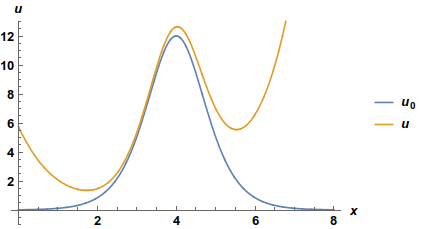
\includegraphics[width=\textwidth]{triv005}
    \caption{График решения при $\ep = 0.05$}
\end{figure}
\begin{figure}[H]
    \centering
    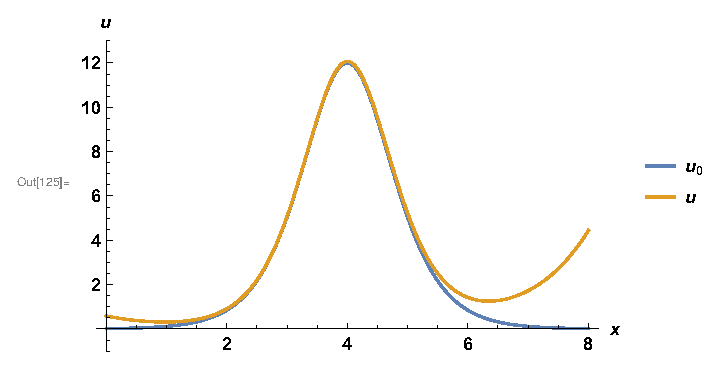
\includegraphics[width=\textwidth]{triv0005}
    \caption{График решения при $\ep = 0.005$}
\end{figure}
\begin{figure}[H]
    \centering
    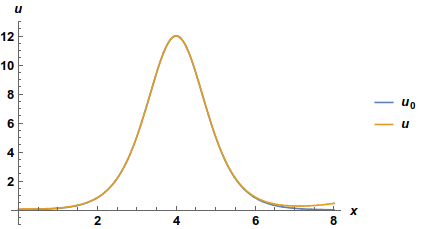
\includegraphics[width=\textwidth]{triv00005}
    \caption{График решения при $\ep = 0.0005$}
\end{figure}

Из рисунков видно, что при $\ep \to 0$
решение $u$ стремится к решению невозмущённого уравнения КдВ.

\section*{Выводы}
\addcontentsline{toc}{section}{Выводы}

Многие задачи прикладной математики, физики
и других областей не позволяют получить точные аналитические решения.
Для получения информации о решениях приходится обращаться к аппроксимации,
численным решениям или к их сочетанию.
Методы асимптотических разложений и
многих масштабов позволяют получить решения с приемлемой точностью.

\clearpage

\bibliographystyle{parts/utf8gost71u}
\bibliography{parts/citations}

\end{document}

